\documentclass[12pt,a4paper]{report}

\usepackage[a4paper,margin=1in]{geometry}
\usepackage[T1]{fontenc}
\usepackage[utf8]{inputenc}
\usepackage{lmodern}
\usepackage{setspace}
\usepackage{titlesec}
\usepackage{fancyhdr}
\usepackage{lastpage}
\usepackage{graphicx}
\usepackage{xcolor}
\usepackage{booktabs}
\usepackage{longtable}
\usepackage{array}
\usepackage{tabularx}
\usepackage{enumitem}
\usepackage{hyperref}
\usepackage{amsmath,amssymb}
\usepackage{tikz}
\usepackage{eso-pic}
\usepackage{caption}
\usepackage{float}
\usepackage{listings}
\usepackage{multirow}
\usepackage{url}

\hypersetup{
    colorlinks=true,
    linkcolor=blue!60!black,
    urlcolor=blue!60!black,
    citecolor=blue!60!black,
    pdftitle={Multimodal Interview Intelligence Platform Documentation},
    pdfauthor={Project Team}
}

\onehalfspacing
\setlength{\headheight}{15pt}
\setlength{\parskip}{4pt}
\setlength{\parindent}{0pt}
\setlength{\emergencystretch}{2em}
\raggedbottom

\definecolor{framecolor}{RGB}{30,60,95}
\definecolor{lightgray}{RGB}{245,245,245}
\definecolor{codegray}{RGB}{70,70,70}

\newcolumntype{Y}{>{\raggedright\arraybackslash}X}

\titleformat{\chapter}[display]
  {\normalfont\bfseries\Huge\color{framecolor}}
  {\chaptertitlename\ \thechapter}{20pt}{\Huge}

\pagestyle{fancy}
\fancyhf{}
\fancyhead[L]{Multimodal Interview Intelligence Platform}
\fancyhead[R]{Technical Documentation}
\fancyfoot[L]{Version 1.0}
\fancyfoot[R]{Page \thepage\ of \pageref{LastPage}}
\renewcommand{\headrulewidth}{0.4pt}
\renewcommand{\footrulewidth}{0.4pt}

% Proper page border on every page
\newcommand\PageBorder{%
\begin{tikzpicture}[remember picture,overlay]
\draw[line width=1.1pt,framecolor]
  ($(current page.north west)+(0.85cm,-0.85cm)$)
  rectangle
  ($(current page.south east)+(-0.85cm,0.85cm)$);
\draw[line width=0.35pt,framecolor!60]
  ($(current page.north west)+(1.05cm,-1.05cm)$)
  rectangle
  ($(current page.south east)+(-1.05cm,1.05cm)$);
\end{tikzpicture}%
}
\AddToShipoutPictureBG{\PageBorder}

\lstdefinestyle{pythonstyle}{
  backgroundcolor=\color{lightgray},
  basicstyle=\ttfamily\small\color{codegray},
  breaklines=true,
  breakatwhitespace=true,
  frame=single,
  rulecolor=\color{framecolor!40},
  columns=fullflexible,
  showstringspaces=false
}

\begin{document}

\begin{titlepage}
    \centering
    \vspace*{1.8cm}
    {\Huge\bfseries Multimodal Interview Intelligence Platform\par}
    \vspace{0.8cm}
    {\LARGE Comprehensive Technical Documentation\par}
    \vspace{1.2cm}

    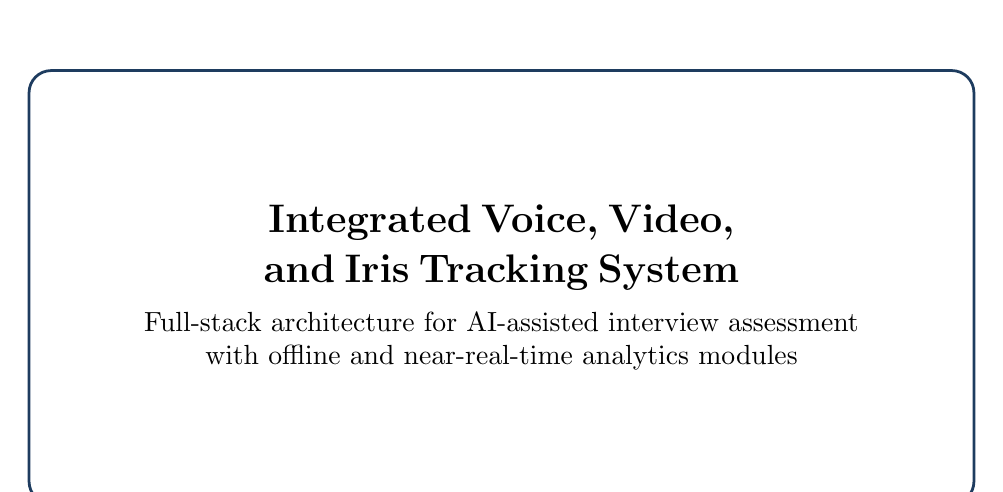
\begin{tikzpicture}
      \draw[rounded corners=8pt, line width=1pt, framecolor] (0,0) rectangle (12,5.5);
      \node[align=center,text width=10.8cm] at (6,2.75) {
        \Large\textbf{Integrated Voice, Video, and Iris Tracking System} \\
        \vspace{0.2cm}
        \normalsize Full-stack architecture for AI-assisted interview assessment \\
        with offline and near-real-time analytics modules
      };
    \end{tikzpicture}

    \vfill

    \begin{tabular}{ll}
        \textbf{Prepared For:} & Engineering and Research Stakeholders \\
        \textbf{Project Root:} & C:/Users/gaura/PRJ \\
        \textbf{Date:} & March 19, 2026 \\
        \textbf{Document Version:} & 1.0
    \end{tabular}

    \vfill

    {\large Internal Technical Report}\par
\end{titlepage}

\pagenumbering{roman}

\chapter*{Executive Summary}
\addcontentsline{toc}{chapter}{Executive Summary}
This project delivers an end-to-end multimodal interview intelligence platform that combines three major sensing and inference capabilities: voice quality scoring, behavioral video scoring, and gaze/iris tracking. The system integrates a modern web frontend, WebSocket-based control flows, Python-based model-serving components, and containerized media infrastructure for interview communication.

The design goal is not only to infer a single aggregate score, but to produce interpretable and operationally useful behavioral signals over time. This includes chunk-level confidence prediction from video, speaking-skill estimation from audio with temporal windows, and gaze-status logging from eye and head signals. The platform is therefore suitable for candidate training scenarios, mock interview simulations, and model experimentation workflows in an applied research setting.

From an architecture perspective, the project combines:
\begin{itemize}[leftmargin=1.5em]
\item A Next.js frontend for interviewer/candidate interaction, chunked capture, and visual diagnostics.
\item FastAPI-based vision orchestration that triggers and aggregates multimodal analyses.
\item Specialized Python modules for video model inference and gaze geometry processing.
\item A dedicated wav2vec-based voice model with regression head for speaking-skill estimation.
\item Dockerized infrastructure for Redis and LiveKit to enable reliable media signaling.
\item Background workers and queue-based flows for scalable asynchronous execution.
\end{itemize}

This documentation provides a complete technical view of the project and separates the Voice Module, Video Module, and Iris Tracking Module into independent sections while also describing how they are fused operationally.

\chapter*{Document Scope and Audience}
\addcontentsline{toc}{chapter}{Document Scope and Audience}
This document is written for machine learning engineers, full-stack developers, MLOps practitioners, QA teams, and project decision-makers who need a full understanding of the implementation and operational model.

\textbf{In scope}
\begin{itemize}[leftmargin=1.5em]
\item System architecture, components, and data flow.
\item Model design and inference pathways for all three core modules.
\item Deployment, runtime controls, diagnostics, and known operational issues.
\item Evaluation strategy and roadmap recommendations.
\end{itemize}

\textbf{Out of scope}
\begin{itemize}[leftmargin=1.5em]
\item Legal policy interpretation for hiring decisions.
\item Production-level cloud hardening beyond current local/experimental deployment.
\item Human factors studies and psychometric validation not yet implemented in code.
\end{itemize}

\tableofcontents
\listoftables
\listoffigures

\cleardoublepage
\pagenumbering{arabic}

\chapter{Project Overview}
\section{Problem Statement}
Interview assessment often depends on human observation quality and can vary between evaluators. This project addresses that challenge by extracting objective multimodal indicators from candidate interactions. Rather than replacing human judgment, the platform assists evaluators with measurable signals related to communication confidence, speaking quality, and visual focus.

\section{Core Objectives}
\begin{itemize}[leftmargin=1.5em]
\item Estimate speaking skill from raw audio waveforms.
\item Estimate confidence and expression-related behavioral signals from interview video.
\item Detect and log gaze orientation/focus status during an interview session.
\item Provide near-real-time updates and final session summaries to the frontend.
\item Support modular experimentation across independently trainable voice and video models.
\end{itemize}

\section{Repository Structure Summary}
The workspace is organized into multiple focused directories including:
\begin{itemize}[leftmargin=1.5em]
\item \textbf{frontend/}: Next.js application and interview UI.
\item \textbf{Vision/}: gaze tracking logic, multimodal orchestration server, and video inference.
\item \textbf{Atempt2/}: training and checkpoints for ranking-supervised video modeling.
\item \textbf{Voice\_Evaluation\_PRJ3/}: wav2vec voice scoring model and analysis scripts.
\item \textbf{backend/} and \textbf{inference-service/}: asynchronous task orchestration and APIs.
\item \textbf{livekit-worker/} and root infra files: communication and runtime support.
\end{itemize}

\begin{figure}[H]
\centering
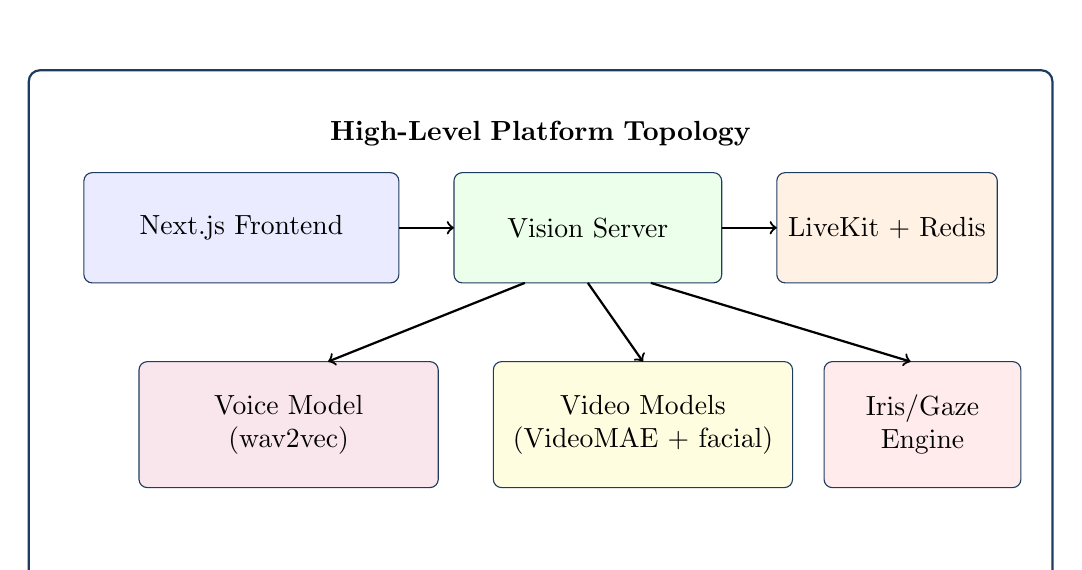
\begin{tikzpicture}
\draw[rounded corners=4pt, line width=0.8pt, framecolor] (0,0) rectangle (13,6.5);
\node[align=center,text width=11.8cm] at (6.5,5.7) {\textbf{High-Level Platform Topology}};
\draw[rounded corners=3pt, fill=blue!8, draw=framecolor] (0.7,3.8) rectangle (4.7,5.2);
\node at (2.7,4.5) {Next.js Frontend};
\draw[rounded corners=3pt, fill=green!8, draw=framecolor] (5.4,3.8) rectangle (8.8,5.2);
\node at (7.1,4.5) {Vision Server};
\draw[rounded corners=3pt, fill=orange!10, draw=framecolor] (9.5,3.8) rectangle (12.3,5.2);
\node at (10.9,4.5) {LiveKit + Redis};
\draw[rounded corners=3pt, fill=purple!10, draw=framecolor] (1.4,1.2) rectangle (5.2,2.8);
\node[align=center] at (3.3,2.0) {Voice Model\\(wav2vec)};
\draw[rounded corners=3pt, fill=yellow!12, draw=framecolor] (5.9,1.2) rectangle (9.7,2.8);
\node[align=center] at (7.8,2.0) {Video Models\\(VideoMAE + facial)};
\draw[rounded corners=3pt, fill=red!8, draw=framecolor] (10.1,1.2) rectangle (12.6,2.8);
\node[align=center] at (11.35,2.0) {Iris/Gaze\\Engine};
\draw[->,thick] (4.7,4.5) -- (5.4,4.5);
\draw[->,thick] (8.8,4.5) -- (9.5,4.5);
\draw[->,thick] (7.1,3.8) -- (7.8,2.8);
\draw[->,thick] (6.3,3.8) -- (3.8,2.8);
\draw[->,thick] (7.9,3.8) -- (11.2,2.8);
\end{tikzpicture}
\caption{Integrated multimodal architecture.}
\end{figure}

\chapter{System Architecture and Runtime Design}
\section{Frontend Layer}
The frontend is implemented in Next.js and provides interview interaction screens, session control, and debug panels. Components such as InterviewRoom, VisionSessionControl, and GazeDebugPanel are designed to:
\begin{itemize}[leftmargin=1.5em]
\item initiate recording or chunk processing,
\item stream or fetch status over WebSocket,
\item display confidence, gaze, and session metrics,
\item expose health and token APIs for media services.
\end{itemize}

Two React hooks define the core communication behavior:
\begin{itemize}[leftmargin=1.5em]
\item \textbf{useVisionSession}: manages a robust WebSocket lifecycle with reconnection, queueing, chunk timeouts, and typed result aggregation.
\item \textbf{useGazeTracking}: supports frame streaming at approximately 30 FPS for continuous gaze inference and calibration commands.
\end{itemize}

\section{Backend and Inference Layer}
The principal orchestration endpoint is a FastAPI-based vision server that handles upload, session initiation, chunk processing, and multimodal response emission. It can spawn subprocesses for offline video processing and also perform in-process model inference for confidence and facial scores.

\textbf{Explicit WebRTC note:} Real-time interview media transport is handled through LiveKit, which is a WebRTC media server. In this project, WebRTC is used for room signaling and real-time audio/video session orchestration between interview participants and the browser clients.

The runtime includes additional support services:
\begin{itemize}[leftmargin=1.5em]
\item Inference service on port 8001 for API-based model jobs.
\item Celery workers with queues for control, chunk inference, and result handling.
\item Redis as a shared queue/cache layer.
\item LiveKit for media signaling and room management.
\end{itemize}

\section{Orchestration Script and Boot Process}
A PowerShell launcher script starts container infrastructure, model services, workers, vision server, and the frontend in separate windows. This design simplifies developer setup and allows module-specific restart cycles during debugging.

\begin{table}[H]
\centering
\caption{Primary runtime endpoints and roles}
\begin{tabularx}{\textwidth}{>{\raggedright\arraybackslash}p{3.0cm} >{\raggedright\arraybackslash}p{2.3cm} Y}
\toprule
\textbf{Component} & \textbf{Default Port} & \textbf{Role} \\
\midrule
Frontend (Next.js) & 3000 & Interview UI, API routes, dashboard rendering \\
Vision Server (FastAPI) & 8000 & Gaze session control, chunk processing, multimodal aggregation \\
Inference Service & 8001 & Additional model API endpoints and inference jobs \\
LiveKit Server & 7880/7881 & WebRTC signaling and room orchestration \\
Redis & 6379 & Queue backend and shared runtime support \\
\bottomrule
\end{tabularx}
\end{table}

\section{End-to-End Runtime Sequence (Detailed)}
The runtime sequence for a typical interview session is as follows:
\begin{enumerate}[leftmargin=1.5em]
\item The candidate enters the interview interface in the frontend and initializes media/session controls.
\item The frontend requests connection credentials and room metadata for LiveKit.
\item LiveKit establishes WebRTC signaling and media channel negotiation with browser peers.
\item In parallel, the frontend maintains WebSocket connectivity to the vision server for analytics control-plane actions.
\item Recorded chunks or uploaded files are transmitted to backend processing endpoints.
\item The vision server executes gaze extraction, video scoring, facial scoring, and voice scoring.
\item Incremental prediction payloads are streamed back to the frontend for progress visibility.
\item Final session aggregates are displayed and can be persisted for later analysis.
\end{enumerate}

Control-plane and media-plane traffic are intentionally separated: WebRTC handles low-latency interview media exchange, while WebSocket/API paths handle analytics orchestration and state synchronization.

\chapter{Video Module (Behavioral Confidence and Facial Analysis)}
\section{Module Purpose}
The Video Module predicts behavioral confidence-like signals from interview recordings and supports additional facial-expression scoring. This module is anchored in the Atempt2 training pipeline and operationalized in the Vision service.

\section{Data and Training Context}
The training logic references RecruitView metadata and video samples. The project timeline indicates iterative optimization for GPU utilization, loader efficiency, and VideoMAE integration. Major changes include mixed precision training, performance-oriented frame loading, and migration to pre-trained VideoMAE backbones.

\section{Modeling Approach}
The video model pipeline can be summarized as:
\begin{enumerate}[leftmargin=1.5em]
\item Sample fixed-length clips (often 16 frames) from each chunk or full video.
\item Preprocess frames using transformer-compatible image processors.
\item Encode temporal-visual representation with VideoMAE backbone.
\item Apply task-specific regression heads for scalar outputs.
\item Produce confidence-like or expression-related predictions.
\end{enumerate}

The model objective used in training is ranking-oriented. The core conceptual objective combines correlation structure and robust pointwise stabilization:
\begin{equation}
\mathcal{L}_{total} = \lambda_{corr}\,\mathcal{L}_{corr}(\hat{y}, y) + \lambda_{huber}\,\mathcal{L}_{huber}(\hat{y}, y)
\end{equation}
where:
\begin{itemize}[leftmargin=1.5em]
\item $\mathcal{L}_{corr}$ encourages ordering consistency with human ranking labels,
\item $\mathcal{L}_{huber}$ regularizes local prediction noise,
\item $\lambda_{corr} \gg \lambda_{huber}$ in ranking-first setups.
\end{itemize}

\section{Inference Strategy}
The realtime inference script supports chunked offline processing of complete recordings:
\begin{itemize}[leftmargin=1.5em]
\item video duration is partitioned into fixed intervals (for example, 15 seconds),
\item each chunk is represented by uniformly sampled frames,
\item model outputs are persisted to JSON after each chunk,
\item summary statistics include min, max, mean confidence and count.
\end{itemize}

This strategy provides incremental visibility even when full-session analysis is still running.

\section{Video Module Outputs}
\begin{table}[H]
\centering
\caption{Video module output schema (simplified)}
\begin{tabularx}{\textwidth}{>{\raggedright\arraybackslash}p{3.2cm} >{\raggedright\arraybackslash}p{2.5cm} Y}
\toprule
\textbf{Field} & \textbf{Type} & \textbf{Description} \\
\midrule
chunk & Integer & Sequential chunk index \\
video\_file & String & Source chunk/video filename \\
confidence & Float & Model output score for chunk \\
timestamp & Float & Unix timestamp at inference completion \\
processing\_time & Float & Inference latency per chunk in seconds \\
\bottomrule
\end{tabularx}
\end{table}

\section{Video Module Engineering Details}
\textbf{Sampling policy.} The module performs uniform frame sampling per chunk to stabilize model behavior across variable frame-rate recordings and to keep tensor shapes deterministic.

\textbf{Checkpoint compatibility.} The inference path supports different checkpoint formats by conditionally resolving either model-only state dictionaries or nested training checkpoints with model keys.

\textbf{Latency behavior.} Chunk-wise processing provides bounded latency windows and enables progressive UI updates. This avoids waiting for complete video completion before surfacing confidence trajectories.

\textbf{Failure handling.} Video-readiness checks and guarded exception paths reduce false failures when files are still being written by recording pipelines.

\section{Operational Strengths and Risks}
\textbf{Strengths}
\begin{itemize}[leftmargin=1.5em]
\item Transfer learning from pre-trained video foundation models.
\item Chunk-wise intermediate output supports UI responsiveness.
\item Mixed-precision path available for CUDA acceleration.
\end{itemize}

\textbf{Risks}
\begin{itemize}[leftmargin=1.5em]
\item Domain shift if interview conditions differ from training distribution.
\item Potential confidence drift with poor lighting or camera quality.
\item Need for explicit calibration of score interpretation for end users.
\end{itemize}

\chapter{Voice Module (Speaking Skills Evaluation)}
\section{Module Purpose}
The Voice Module estimates speaking skill from candidate audio tracks and supports both full-clip and sliding-window analysis. It is implemented under Voice\_Evaluation\_PRJ3 and integrated into the Vision server through a reusable analyzer class.

\section{Architecture}
The module uses transfer learning based on the wav2vec2 base encoder and a regression head for continuous score prediction.

\begin{equation}
\hat{s} = f_{head}(\operatorname{Pool}(f_{wav2vec}(x_{audio})))
\end{equation}

where $x_{audio}$ is a normalized mono waveform sampled at 16 kHz, padded or clipped to a configured max duration.

\section{Preprocessing and Input Constraints}
\begin{itemize}[leftmargin=1.5em]
\item Input can be audio or video; non-WAV assets are converted through ffmpeg.
\item Stereo inputs are collapsed to mono.
\item Waveform length is normalized to a fixed-duration tensor.
\item Inference path is device-aware and uses CUDA if available.
\end{itemize}

\section{Temporal Behavior Analytics}
Beyond a single score, the voice module computes windowed trends using fixed-size windows and stride. This provides a timeline that can reveal whether speaking performance is stable, improving, or degrading during an interview.

In addition, lightweight signal features are extracted:
\begin{itemize}[leftmargin=1.5em]
\item energy proxy from moving RMS,
\item pitch-proxy signals,
\item optional zero-crossing characteristics for voicing dynamics.
\end{itemize}

\section{Training Pipeline Characteristics}
The training script uses supervised regression with Huber loss, Adam optimization, and mini-batch loaders. The pipeline emphasizes practical robustness over over-parameterized tuning and supports fast iteration for dataset and head adjustments.

\section{Voice Module Output Contract}
\begin{table}[H]
\centering
\caption{Voice analysis output schema (simplified)}
\begin{tabularx}{\textwidth}{>{\raggedright\arraybackslash}p{3.2cm} >{\raggedright\arraybackslash}p{2.5cm} Y}
\toprule
\textbf{Field} & \textbf{Type} & \textbf{Description} \\
\midrule
score & Float or null & Overall speaking score \\
window\_times & Array[Float] & Start times for sliding windows \\
window\_scores & Array[Float] & Predicted score per window \\
energy & Array[Float] & Energy proxy timeline \\
pitch\_proxy & Array[Float] & Pitch-related trend proxy \\
error & String or null & Error details if inference fails \\
\bottomrule
\end{tabularx}
\end{table}

\section{Voice Module Engineering Details}
\textbf{Model lifecycle.} The voice model is loaded once and reused across requests, reducing repeated initialization overhead and improving throughput for chunk workloads.

\textbf{Audio normalization contract.} Every input is converted to a stable format (mono, 16 kHz, fixed max duration), ensuring predictable input statistics for inference.

\textbf{Temporal explainability.} Sliding-window inference captures local speaking variability and supports diagnostics beyond a single clip-level scalar score.

\textbf{Operational fallback.} If the voice model is unavailable or conversion fails, structured error payloads are returned so the session can proceed with remaining modalities.

\section{Operational Strengths and Risks}
\textbf{Strengths}
\begin{itemize}[leftmargin=1.5em]
\item Leverages rich speech representations from pretrained foundation model.
\item Produces both aggregate and temporal scores.
\item Handles multiple input formats via deterministic conversion path.
\end{itemize}

\textbf{Risks}
\begin{itemize}[leftmargin=1.5em]
\item Environmental noise and recording devices can alter score stability.
\item Accent, language, and speaking-style variability may introduce bias.
\item Long pauses and clipped speech may reduce reliability.
\end{itemize}

\section{Iris Tracking Engineering Details}
\textbf{Geometric interpretation.} The gaze engine approximates viewing direction by combining facial landmarks, head orientation cues, and a monitor-plane model. This supports interpretable status labels and screen-coordinate estimates.

\textbf{Calibration effects.} Screen calibration and marker updates improve relative accuracy by adapting mapping offsets to user posture and camera placement.

\textbf{Headless execution.} A headless mode is available for service environments where OpenCV windows are not desired, while debug modes remain available for development calibration.

\textbf{Robustness constraints.} Tracking quality is sensitive to occlusions, extreme head angles, and low-light conditions, and therefore should be interpreted as behavioral signal support rather than deterministic truth.

\chapter{Iris Tracking Module (Gaze and Attention Monitoring)}
\section{Module Purpose}
The Iris Tracking Module is centered around the Vision gaze engine and provides detailed per-frame focus signals, calibration workflows, and session logs. It is designed for interview engagement analysis rather than medical-grade eye-tracking.

\section{Pipeline Overview}
The implementation uses computer vision geometry and facial landmarks to estimate head orientation, eye direction, and inferred gaze status. The module supports:
\begin{itemize}[leftmargin=1.5em]
\item webcam or uploaded video input,
\item headless and windowed debug modes,
\item screen calibration and marker-based refinement,
\item event logging with timestamps and qualitative status labels.
\end{itemize}

\section{Calibration and Coordinate Logic}
The module constructs an approximate monitor plane in world coordinates and estimates gaze intersection points. Conceptually:
\begin{equation}
\mathbf{p}_{gaze}(t) = \mathbf{o} + t\,\mathbf{d}
\end{equation}
where $\mathbf{o}$ is the gaze origin and $\mathbf{d}$ is the normalized gaze direction. Intersection with a monitor plane approximates on-screen focus location.

Status labels such as Looking Forward, Looking Away, Eyes Away, or No Face Detected are generated from thresholded angular and visibility checks.

\section{Frontend Debug and Control Integration}
The frontend exposes:
\begin{itemize}[leftmargin=1.5em]
\item connection status, calibration status, and FPS counters,
\item real-time screen coordinates and marker count,
\item controls for screen calibration, marker insertion, and reset,
\item timeline-style display of recent gaze events.
\end{itemize}

\section{Session Metric Derivations}
A simple focus percentage can be computed as:
\begin{equation}
\text{Focus\%} = \frac{N_{focused}}{N_{total}} \times 100
\end{equation}
where focused events exclude away-status entries.

This metric is useful as a first-level indicator but should be interpreted alongside confidence and voice trends.

\section{Operational Strengths and Risks}
\textbf{Strengths}
\begin{itemize}[leftmargin=1.5em]
\item Real-time and offline usage options.
\item Rich debug telemetry for calibration verification.
\item Transparent status labels suitable for user feedback loops.
\end{itemize}

\textbf{Risks}
\begin{itemize}[leftmargin=1.5em]
\item Lighting variation and webcam quality sensitivity.
\item Head pose extremes can destabilize eye-only metrics.
\item Requires careful communication to avoid over-interpretation.
\end{itemize}

\chapter{Cross-Module Fusion and Session Flow}
\section{Unified Chunk Processing Workflow}
For chunked interview operation, the frontend records or references chunk assets and sends process requests via WebSocket. The backend then executes gaze extraction, video confidence inference, facial scoring, and voice analysis in coordinated steps.

\begin{enumerate}[leftmargin=1.5em]
\item Frontend emits process\_chunk action with video path and chunk IDs.
\item Vision server validates file readiness and dispatches analyzers.
\item Gaze log, video prediction, facial score, and voice result are collected.
\item A chunk\_processed message is returned with merged payload.
\item Frontend updates live cards, trend plots, and session aggregates.
\end{enumerate}

\section{WebSocket Reliability Design}
The hook implementation includes critical robustness patterns:
\begin{itemize}[leftmargin=1.5em]
\item exponential backoff reconnection,
\item outbound message queue when socket is not open,
\item per-chunk timeout guards for stalled jobs,
\item state partitioning for active, completed, and failed chunks.
\end{itemize}

\section{Result Harmonization Strategy}
Because each modality has different temporal granularity and confidence characteristics, the current design keeps modality outputs independent and display-oriented. A future fusion layer can normalize and calibrate each score stream before producing any composite KPI.

\chapter{APIs, Contracts, and Data Schemas}
\section{Vision Server Actions (WebSocket)}
Representative control actions include:
\begin{itemize}[leftmargin=1.5em]
\item start\_session with video path,
\item stop\_session,
\item process\_chunk with chunk metadata,
\item status polling and session updates.
\end{itemize}

\section{Event Types Returned to Frontend}
Typical event messages:
\begin{itemize}[leftmargin=1.5em]
\item session\_started,
\item prediction\_update,
\item prediction\_summary,
\item chunk\_processed,
\item chunk\_error,
\item session\_ended,
\item error.
\end{itemize}

\section{Chunk Payload Structure}
\begin{lstlisting}[style=pythonstyle,caption={Abstract chunk-processed payload shape}]
{
  "type": "chunk_processed",
  "chunk_id": "uuid",
  "chunk_index": 3,
  "gaze_data": [...],
  "predictions": [...],
  "inference_summary": {
    "count": 1,
    "mean_confidence": 0.62,
    "min_confidence": 0.62,
    "max_confidence": 0.62
  },
  "voice_analysis": {
    "score": 0.57,
    "window_times": [0,2,4],
    "window_scores": [0.55,0.58,0.60],
    "error": null
  },
  "facial_analysis": {
    "score": 0.64,
    "error": null
  }
}
\end{lstlisting}

\chapter{Deployment, Operations, and Troubleshooting}
\section{Local Deployment Pattern}
The project currently follows a local-first deployment model:
\begin{itemize}[leftmargin=1.5em]
\item Docker Compose brings up Redis and LiveKit.
\item PowerShell orchestration starts inference APIs and workers.
\item Vision server is launched under a configured conda environment.
\item Next.js frontend is launched in development mode.
\end{itemize}

\textbf{Explicit Dockerization note:} The current implementation is \textit{partially dockerized}. Infrastructure services (Redis and LiveKit/WebRTC) run in Docker containers, while application services (frontend, vision server, inference service, and Celery workers) run directly on the host via Python/Node environments. Therefore, the whole project is not yet fully containerized end-to-end.

\begin{table}[H]
\centering
\caption{Containerization boundary in the current implementation}
\begin{tabularx}{\textwidth}{>{\raggedright\arraybackslash}p{5.0cm} >{\raggedright\arraybackslash}p{3.0cm} Y}
\toprule
\textbf{Component Group} & \textbf{Execution Mode} & \textbf{Current Status} \\
\midrule
Redis + LiveKit (WebRTC media layer) & Docker Compose & Containerized \\
Frontend (Next.js) & Host process (npm) & Not containerized \\
Vision server (FastAPI) & Host process (conda/python) & Not containerized \\
Inference service + Celery workers & Host process (conda/python) & Not containerized \\
\bottomrule
\end{tabularx}
\end{table}

\section{Full Dockerization Blueprint (Planned)}
To move from partial to full containerization, the recommended next architecture is:
\begin{enumerate}[leftmargin=1.5em]
\item Add Dockerfiles for frontend, vision server, inference service, and worker runtime.
\item Convert the startup PowerShell orchestration into Docker Compose services with explicit dependencies.
\item Externalize environment variables using Compose env files and secret management.
\item Attach all services to a common bridge network with stable service names.
\item Add health checks for each service and restart policies for resilience.
\item Optionally add a reverse proxy service for unified ingress and TLS termination.
\end{enumerate}

This approach would make the project reproducible across developer and CI environments while reducing machine-specific setup drift.

\section{LiveKit Connectivity Considerations}
The troubleshooting guide highlights common failure classes:
\begin{itemize}[leftmargin=1.5em]
\item missing environment keys,
\item unavailable media server container,
\item token-generation misconfiguration,
\item local port conflicts.
\end{itemize}

\section{Operational Checklist}
\begin{enumerate}[leftmargin=1.5em]
\item Validate frontend environment variables for LiveKit URL and keys.
\item Confirm Docker containers are running and healthy.
\item Confirm token endpoint responds with valid payload.
\item Confirm WebSocket endpoint for vision server is reachable.
\item Run interview page and verify debug panels for module status.
\end{enumerate}

\chapter{Evaluation Framework and Quality Strategy}
\section{Recommended Metrics by Module}
\begin{table}[H]
\centering
\caption{Validation metrics by modality}
\begin{tabularx}{\textwidth}{>{\raggedright\arraybackslash}p{2.8cm} >{\raggedright\arraybackslash}p{3.0cm} Y}
\toprule
\textbf{Module} & \textbf{Core Metrics} & \textbf{Purpose} \\
\midrule
Video & Spearman, Kendall, temporal stability & Rank consistency and chunk reliability \\
Voice & MAE, Spearman, window variance & Overall and time-local speaking assessment quality \\
Iris Tracking & Focus ratio, away-event rate, FPS stability & Attention consistency and runtime robustness \\
Cross-module & Missing-rate, latency, agreement analysis & Fusion-readiness and operational quality \\
\bottomrule
\end{tabularx}
\end{table}

\section{Offline and Online Test Strategy}
\textbf{Offline tests}
\begin{itemize}[leftmargin=1.5em]
\item deterministic model input-output checks,
\item schema validation for serialized outputs,
\item stress tests on long recordings and short/empty chunks.
\end{itemize}

\textbf{Online tests}
\begin{itemize}[leftmargin=1.5em]
\item WebSocket reconnect scenarios,
\item degraded network behavior,
\item simultaneous chunk processing under worker load,
\item UI consistency across partial failures.
\end{itemize}

\section{Latency Budgeting Considerations}
Define service-level targets for chunk turnaround and UI refresh. A practical baseline is to keep median chunk processing time below chunk duration for a near-real-time user experience in mock interviews.

\chapter{Security, Privacy, and Responsible Use}
\section{Data Sensitivity}
Audio, video, and gaze trajectories are personally identifiable behavioral data. Therefore:
\begin{itemize}[leftmargin=1.5em]
\item capture consent explicitly,
\item avoid storing raw media longer than necessary,
\item encrypt data at rest in production deployments,
\item separate research and operational data domains.
\end{itemize}

\section{Responsible Scoring Principles}
Predictions must be presented as assistive analytics, not sole decision criteria. Human-in-the-loop review and bias monitoring are required before using outputs in any evaluative context.

\section{Model Governance Recommendations}
\begin{itemize}[leftmargin=1.5em]
\item keep versioned model cards for each checkpoint,
\item maintain data lineage for training and validation splits,
\item log confidence intervals or uncertainty proxies where possible,
\item enforce periodic recalibration and drift checks.
\end{itemize}

\chapter{Roadmap and Improvement Plan}
\section{Short-Term (0-2 months)}
\begin{itemize}[leftmargin=1.5em]
\item standardize schemas for all analyzer outputs,
\item improve chunk-level retry and idempotency,
\item add structured benchmark scripts and CI checks,
\item enrich frontend result visualization for temporal explainability.
\end{itemize}

\section{Mid-Term (2-6 months)}
\begin{itemize}[leftmargin=1.5em]
\item introduce calibrated multimodal fusion layer,
\item add experiment tracking for hyperparameters and checkpoints,
\item harden production deployment with secret management and observability,
\item add automated fairness diagnostics by subgroup.
\end{itemize}

\section{Long-Term (6+ months)}
\begin{itemize}[leftmargin=1.5em]
\item active learning loops for model improvement,
\item adaptive interview coaching interventions,
\item cloud-scale orchestration with autoscaling inference,
\item formal validation studies with external evaluators.
\end{itemize}

\chapter{Conclusion}
This project establishes a robust foundation for multimodal interview analytics by combining independent yet interoperable modules for video behavior scoring, voice quality evaluation, and iris/gaze tracking. The architecture is practical for iterative experimentation and already includes many engineering elements needed for reliable operation: service orchestration, diagnostics, typed frontend hooks, chunk-wise workflows, and deployable infrastructure.

The clear separation of modules allows independent innovation while preserving end-to-end compatibility. With additional calibration, governance, and scale hardening, this platform can evolve from a research-grade system into a production-ready interview intelligence stack.

\appendix

\chapter{Appendix A: Environment and Service Start Commands}
\begin{lstlisting}[style=pythonstyle,caption={Representative startup sequence on Windows PowerShell}]
# From project root
cd C:/Users/gaura/PRJ

# Start infra
Docker compose up -d

# Start inference service (Conda env example: pupil310)
conda run --no-capture-output -n pupil310 uvicorn main:app --host 0.0.0.0 --port 8001

# Start worker
conda run --no-capture-output -n pupil310 celery -A backend.worker.celery_app worker -l info

# Start vision server
conda run --no-capture-output -n pupil310 python Vision/vision_server.py

# Start frontend
cd frontend
npm run dev
\end{lstlisting}

\chapter{Appendix B: Suggested Overleaf Usage}
\begin{enumerate}[leftmargin=1.5em]
\item Create a new Overleaf project.
\item Replace main.tex with this document content.
\item Compile using pdfLaTeX.
\item If needed, reduce font to 11pt or adjust spacing to hit a target page range.
\item Insert real screenshots and architecture diagrams where placeholders exist.
\end{enumerate}

\end{document}
